\section{Implicações para o desenho da reforma}\label{sec:policy}

O objeto relevante de política não é apenas a versão original de 36 horas da PEC 8/2025. O debate legislativo de 2025 e abril de 2026 também inclui alternativas de 40 horas, escala 5x2 e transições faseadas. Por isso, o modelo calcula a sequência completa de tetos de horas, e não apenas o endpoint mais intenso.

Um teto de 40 horas é uma reforma moderada nessa aritmética. Na base formal limitada inicialmente a 44h e sob a calibração central de eficiência, ele exige $1{,}53$--$1{,}57\%$ de PTF para restaurar o produto e deixa positivo o indicador GHH representativo. O movimento para 36 horas é maior: afeta $85{,}6\%$ dos trabalhadores formais e exige um salto único de produtividade entre $6{,}52\%$ sob fadiga só acima de 40h e $8{,}38\%$ sob penalidade bilateral. O apêndice mostra como essas magnitudes mudam com a eficiência e a distribuição inicial de horas.

Os requisitos de 36 horas são grandes quando lidos como benchmark de escala contra o histórico brasileiro pós-1990. Na PWT 11.0, a PTF brasileira cai de 1990 a 2023 e também no horizonte pré-Covid de 1990 a 2019. Mesmo a melhor década móvel inteiramente contida em 1990--2019, de 2000 a 2010, cresce apenas $+0{,}05\%$ ao ano. Em um horizonte de cinco anos, o requisito de 36h sob fadiga só acima de 40h equivale a $1{,}27\%$ ao ano de PTF, enquanto o de 40h equivale a $0{,}30\%$ ao ano. Essa comparação não prova inviabilidade; ela apenas coloca o tamanho do ganho requerido na escala da experiência recente brasileira.

A curva é inclinada. O teto de 40 horas mantém o requisito abaixo daquele associado a 36 horas nas especificações examinadas. Mover diretamente para 36 horas impõe uma exigência elevada de produtividade pelo padrão brasileiro pós-1990. Sem esse salto, o modelo produz perda de produto de curto prazo de $6{,}65$ a $8{,}40$ por cento na base principal. O requisito de produtividade é uma referência contábil, não uma previsão.

Uma redução moderada do teto eleva o indicador GHH dentro da calibração central do modelo porque o valor atribuído ao lazer adicional supera o consumo perdido. Em 40 horas, o equivalente de consumo é de $+0{,}18\%$ sob penalidade bilateral e $+0{,}22\%$ sob fadiga só acima do pico. Em 36 horas, ambas as funções produzem perda de bem-estar representativo: $-3{,}42\%$ e $-1{,}66\%$, respectivamente, em equivalente de consumo. A interpretação exige separar produto, PTF requerida e bem-estar: uma redução moderada pode reduzir o produto, elevar o bem-estar representativo e ainda exigir um ganho de PTF positivo. O diagnóstico permanece dependente das hipóteses de fadiga e de mensuração das horas.

O requisito no endpoint varia entre setores. A indústria carrega o maior requisito em 36 horas: $8{,}97\%$ sob eficiência bilateral, próxima da agricultura ($8{,}85\%$) e acima dos serviços ($8{,}16\%$). Todos os três setores veem a informalidade subir. Os serviços concentram a maior parte da perda agregada de produto via sua escala de produto: cerca de $66\%$ a $67\%$ em 36 horas na extensão setorial, conforme a função de eficiência. O exercício setorial é de equilíbrio parcial, setor por setor, e não uma análise insumo-produto de incidência.

A informalidade sobe, mas não explica a maior parte da perda de produto. O modelo calibrado pela razão de remuneração horária formal--informal encontra um aumento agregado de informalidade de $2{,}28$ a $2{,}92$ p.p. em 36 horas. A decomposição mostra que o custo de produto vem sobretudo de menos horas trabalhadas. Ainda assim, a reforma desloca empregos adicionais para a informalidade, enfraquecendo os objetivos formalizadores da política.

A Figura~\ref{fig:transition_map} compara os pacotes de transição nas alternativas de 44 para 40 horas (painel A) e de 44 para 36 horas (painel B). Ela cruza a substituição formal--informal, medida por $\sigma$, com a redução do custo de formalização, usando os mesmos eixos e a mesma escala de cores. Esse custo é o componente privado adicional por emprego formal representado por $\tau$ no modelo. No ponto $\sigma=1{,}326$, reduzi-lo em $10\%$ leva o requisito de PTF de $1{,}573\%$ para $0{,}845\%$ em 40h, mas de $8{,}381\%$ para $7{,}606\%$ em 36h.

A diferença de intensidade aparece ao fixar o objetivo de preservar o produto. Em 40h, uma redução de $23{,}53\%$ nesse custo é suficiente para zerar $\Areq$ na calibração central. Em 36h, mesmo eliminar inteiramente esse componente deixa um requisito de PTF de $4{,}62\%$. Portanto, a transição para 36h exige, nesse exercício, ganhos de produtividade além da redução do custo de formalização. O mapa compara custos privados; não identifica o orçamento de um pacote fiscal, sua focalização por porte ou os efeitos de um subsídio temporário.

\begin{figure}[p]
\centering
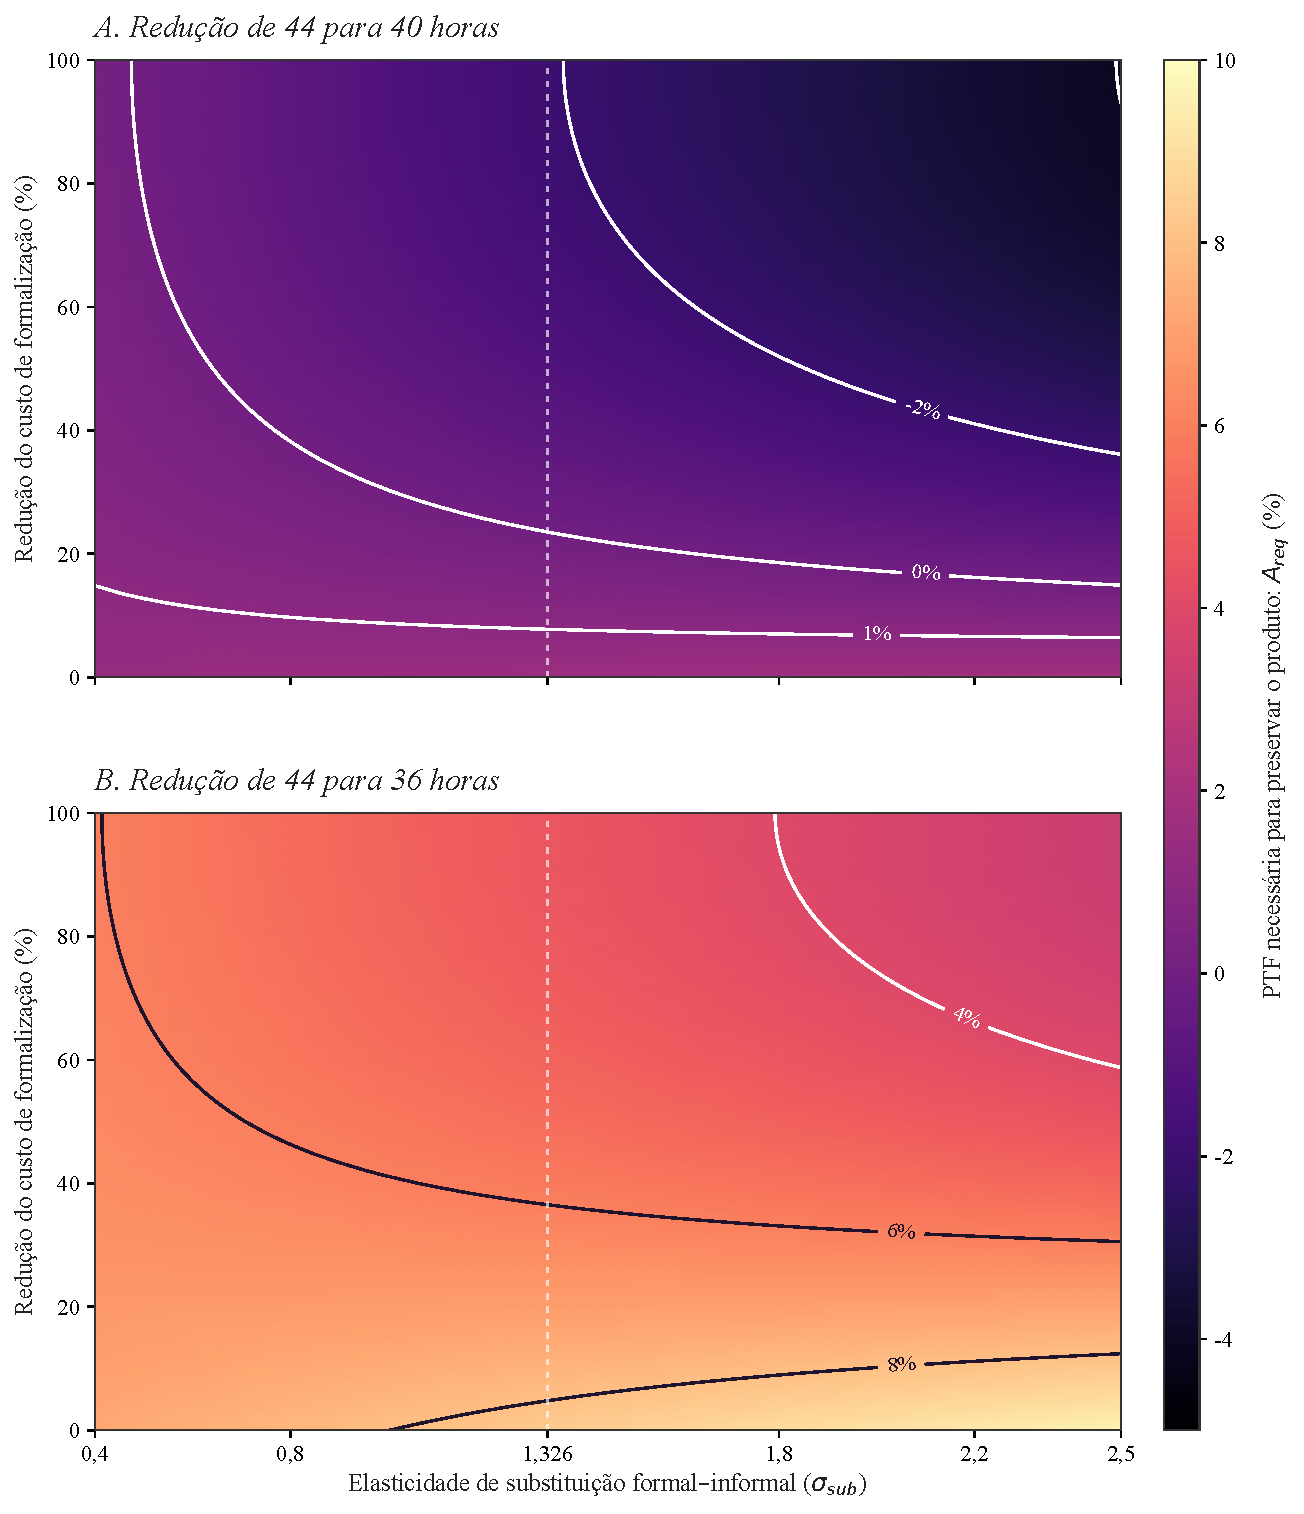
\includegraphics[width=0.94\textwidth]{generated/fig_transition_map_pt.pdf}
\caption{Produtividade requerida e redução do custo de formalização: de 44 para 40h (A) e de 44 para 36h (B).}\label{fig:transition_map}
\tabnotes{Ambos os painéis partem da mesma base formal limitada a 44h, com eficiência bilateral e um grupo nacional. O eixo vertical mostra $100r$, em $\tau^{cap}=(1-r)\tau$: $100\%$ elimina o custo adicional $\tau$ do modelo, sem representar uma alíquota fiscal. Para cada $\sigma$, recalibram-se a ponte horária e os custos no estado inicial; depois se reduz somente $\tau$, mantendo $\pi$, capital e âncora de ajuste. Cores e isocurvas usam a mesma escala de $\Areq$, com composição reotimizada em cada avaliação de PTF. Valores negativos correspondem a ganho de produto sob a PTF inicial. A linha vertical tracejada marca $\sigma=1{,}326$. Os painéis são alternativas à base de 44h, não etapas de uma trajetória dinâmica.}
\end{figure}

\paragraph{Por que um pacote de transição importa?} A diferença entre 40 e 36 horas motiva a discussão de instrumentos que facilitem a reorganização do trabalho durante a implementação. Evidência recente de pilotos de semana de quatro dias ajuda a situar essa margem: \citet{FanSchorKellyGu2025} analisam uma intervenção de seis meses em 141 organizações e 2.896 trabalhadores em seis países, com redução de jornada sem corte salarial, e encontram melhora em burnout, satisfação, saúde mental e saúde física. A capacidade de trabalho é autorreportada; o estudo não estima PTF agregada. Esse resultado deve ser lido como evidência de viabilidade organizacional e bem-estar, de modo que complementa, mas não substitui, a aritmética de $\Areq$. A calibração não quantifica o efeito de um pacote fiscal: isso exigiria identificar as cunhas e seu financiamento.

O modelo é de curto prazo e equilíbrio parcial. Capital e emprego total são mantidos fixos, de modo que o modelo desliga investimento e partilha de trabalho. Decisões de investimento e custos de ajuste do capital, discutidos por \citet{Caballero1999}, constituem uma margem adicional para extensões dinâmicas. A evidência sobre partilha de trabalho na Alemanha \citep{Hunt1996} e na reforma constitucional brasileira de 1988 \citep{GonzagaMenezesFilhoCamargo2003}, assim como a experiência portuguesa de 1996 \citep{AsaiLopesTondini2024}, fornece contexto para essas margens, com os limites de comparação discutidos na Seção~\ref{sec:validation}.

Sob esses limites, a aritmética da produtividade motiva a avaliação de caminhos faseados. Uma parada intermediária em 40 horas mantém o requisito de produtividade abaixo do endpoint de 36 horas; o ganho do calendário de transição em si, porém, exige uma análise dinâmica. A implicação é condicional ao modelo: a intensidade da redução e a resposta da produtividade importam para a aritmética de produto e para o indicador de consumo--lazer representativo.

\FloatBarrier
